
\section{Validation}
\label{repl:sec:validation}


\subsection{Référence}

\begin{figure}
  \begin{center}
    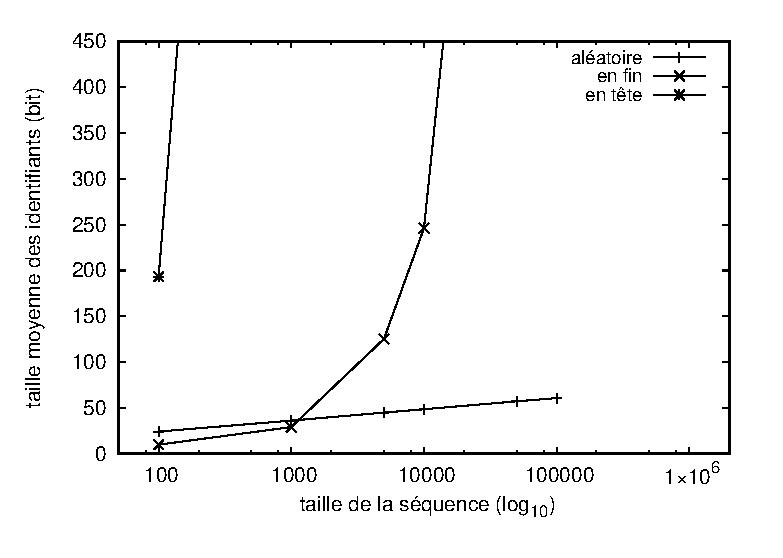
\includegraphics[width=0.8\textwidth]{img/lseq/logoot.eps}
    \caption{\label{repl:img:logoot} Arbre à arité constante avec stratégie
      d'allocation adaptée à l'édition en fin. L'axe des abscisses montre la
      taille du document sur une échelle logarithmique en base décimale. L'axe
      des ordonnées montre la moyenne des tailles des chemins alloués.}
  \end{center}
\end{figure}


\subsection{Arbre exponentiel}

\begin{figure}
  \centering
  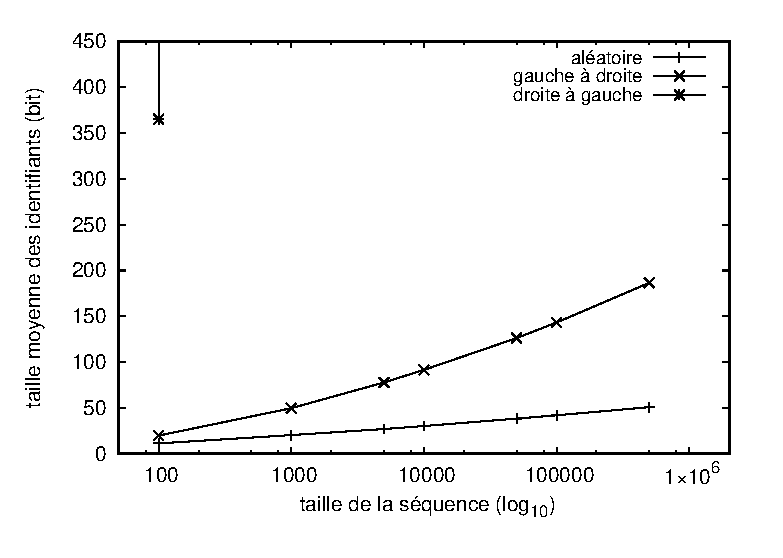
\includegraphics[width=0.8\textwidth]{img/lseq/double.eps}
  \caption{\label{repl:img:exponentialtree} Arbre exponentiel avec stratégie
    d'allocation adaptée à l'édition en fin. L'axe des abscisses montre la
    taille du document sur une échelle logarithmique en base décimale. L'axe des
    ordonnées montre la moyenne des tailles des chemins alloués.}
\end{figure}

\paragraph{Objectif :} Montrer que le chemin des identifiants alloués progresse
de manière sous-linéaire par rapport à la taille du document. Montrer que
lorsque le comportement d'édition va à l'opposé de celui prévu, l'allocation
devient désastreuse.

\paragraph{Description :} Des documents sont créés artificiellement par
insertions successives de caractères. Trois types de comportement d'édition sont
simulés :
\begin{inparaenum}[(i)]
\item à des positions aléatoire dans le document,
\item à la fin,
\item en tête.
\end{inparaenum}
La moyenne de la taille des identifiants est mesurée à 100, 1k, 5k, 10k, 50k,
100k, 500k insertions. La structure utilisée est celle d'un arbre exponentiel
dont l'arité maximale de départ est fixée à $2^5$.

\paragraph{Résultat :} La figure~\ref{repl:img:exponentialtree} montre les
résultats des mesures effectuées pendant la simulation. Nous observons que lors
de l'édition en position aléatoire, l'allocation se comporte extrêmement bien
avec des chemins de taille logarithmique. Lors de l'édition en fin, la taille
moyenne des chemins suit une augmentation sous-linéaire par rapport au nombre
d'insertions dans le document. Finalement, l'édition en tête entraine une très
forte augmentation de la taille des identifiants.

\paragraph{Explication :} L'édition aléatoire place les éléments au hazard dans
la séquence. L'arbre est équilibré car nulle branche n'est remplie en
particulier. À terme, toutes les branches les plus basses sont remplies. Dans ce
cas, les chemins sont de taille moyenne logarithmiques ce qui constitue la borne
minimale. Lors de l'édition en queue, les chemins les plus à gauche sont alloués
réservant de l'espace aux insertions futures. De plus, puisque l'arité de
l'arbre double à chaque niveau, il peut accueillir deux fois plus de chemins à
un prix minime (+1 bit/niveau). Pour cette même raison, l'allocation est
désastreuse lors de l'édition en tête : Quelques insertions suffisent à faire
augmenter la profondeur de l'arbre. L'arité maximale augmente alors rapidement
et le prix des identifiants explose.


\subsection{Sous-fonctions d'allocation}

\begin{figure}
  \centering
  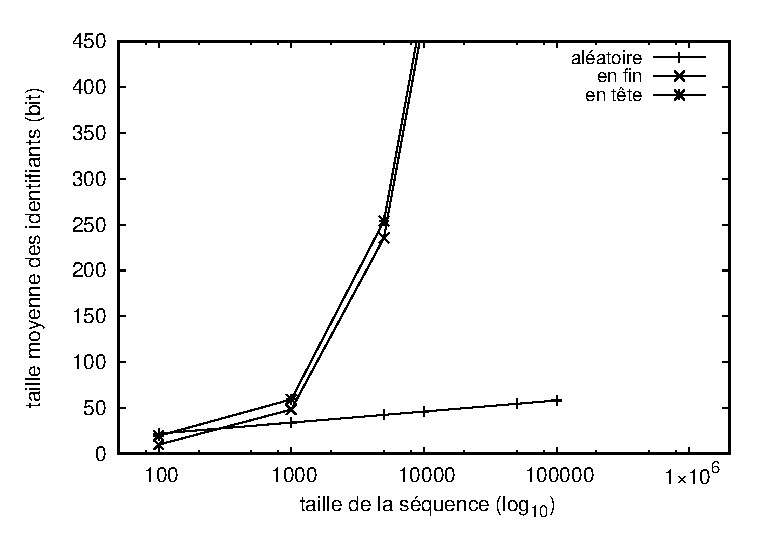
\includegraphics[width=0.8\textwidth]{img/lseq/robin.eps}
  \caption{\label{repl:img:suballocation} Arbre à arité constante et deux
    sous-stratégies d'allocation. L'axe des abscisses montre la taille du
    document sur une échelle logarithmique en base décimale. L'axe des ordonnées
    montre la moyenne des tailles des chemins alloués.}
\end{figure}

\paragraph{Objectif :} Montrer que deux sous-fonctions d'allocation conçues avec
des objectifs antagonistes mais utilisées ensemble gèrent les comportements
d'édition triviaux. Montrer que la progression des identifiants reste linéaire
comparé à la taille du document.

\paragraph{Description :} La simulation concerne trois documents grossissant au
rythme des opérations d'insertions effectuées respectivement en tête, en fin, et
aléatoirement. L'arbre a une arité maximale constante. Chaque niveau se voit
attribuer une sous-fonction d'allocation, i.e., les niveaux pairs avec une
fonction adaptée à l'édition en tête, et les niveaux impairs avec une fonction
adaptée à l'édition en fin. Nous mesurons la moyenne des chemins composant les
identifiants à 100, 1k, 5k, 10k, 50k, 100k insertions.

\paragraph{Résultat :} La figure~\ref{repl:img:suballocation} montre les
résultats obtenus à la suite de ces simulations. Nous observons tout d'abord que
les chemins reste logarithmique sous un comportement d'édition aléatoire. Nous
observons aussi que pour l'édition en tête et l'édition en fin, la progression
est linéaire mais surtout, quasiment identique dans les deux cas.

\paragraph{Explication :} Tout comme pour la
figure~\ref{repl:img:exponentialtree}, l'édition à des positions aléatoire à
pour effet d'équilibrer l'arbre représentant le document répliqué. Les chemins
résultant de ce comportement grandissent de manière logarithmique. Grâce à une
alternance des sous-fonctions d'allocation, la taille des chemins alloués lors
de l'édition en tête ou en fin augmente lentement. Malgré tout, la progression
reste linéaire. De plus, elle augmente deux fois plus rapidement que sans cette
alternance avec un comportement d'édition favorable. En effet, dans le cas de
ces simulations, un niveau sur deux composant un chemin est perdu car consommé
trop vite : la sous-fonction d'allocation assignée à ce niveau n'était pas celle
conçue pour le comportement d'édition courant.


\subsection{Arbre exponentiel et sous-fonctions}

\begin{figure}
  \begin{center}
    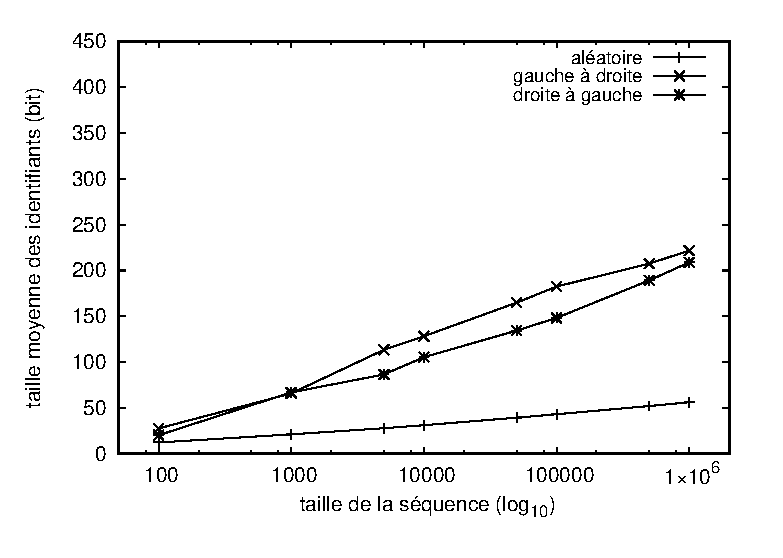
\includegraphics[width=0.8\textwidth]{img/lseq/lseq.eps}
    \caption{\label{repl:img:lseq} Arbre exponentiel avec deux sous-stratégies
      d'allocation. L'axe des abscisses montre la taille du document sur une
      échelle logarithmique en base décimale. L'axe des ordonnées montre la
      moyenne des tailles des chemins alloués.}
  \end{center}
\end{figure}
